\documentclass[varwidth=true, border=2pt]{standalone}
\usepackage{tikz}
\usetikzlibrary{patterns}

\begin{document}
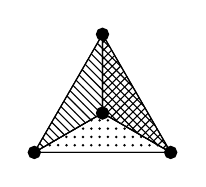
\begin{tikzpicture}
    \tikzstyle{point}=[circle,thick,draw=black,fill=black,inner sep=0pt,minimum width=4pt,minimum height=4pt]
    \node (z)[point] at (0,0) {};
    \node (a)[point] at (90:1cm) {};
    \node (b)[point] at (210:1cm) {};
    \node (c)[point] at (330:1cm) {};
    \path (z.center) edge (a.center);
    \path (z.center) edge (b.center);
    \path (z.center) edge (c.center);
    \draw (a.center) -- (b.center) -- (c.center) -- cycle;

    \draw[pattern=north west lines] (a.center) -- (b.center) -- (z.center) --cycle;
    \draw[pattern=dots] (b.center) -- (c.center) -- (z.center) --cycle;
    \draw[pattern=crosshatch] (a.center) -- (c.center) -- (z.center) --cycle;
\end{tikzpicture}
\end{document}
